\documentclass{article}
\usepackage[utf8]{inputenc}
\usepackage{float}
\usepackage[english]{babel}
\setlength{\oddsidemargin}{0.25 in}
\setlength{\evensidemargin}{-0.25 in}
\setlength{\topmargin}{-0.6 in}
\setlength{\textwidth}{6.5 in}
\setlength{\textheight}{8.5 in}
\setlength{\headsep}{0.75 in}
\setlength{\parindent}{0 in}
\setlength{\parskip}{0.1 in}
\usepackage{xspace}
\usepackage{comment}
\usepackage{amssymb, amsmath, amsfonts, amsthm, graphics, mathrsfs, enumitem, tikz-cd}
\usepackage[hmargin=1 in, vmargin = 1 in]{geometry}
\usepackage{changepage}
\begin{document}
\section{Connectivity conditions for a universal cover}
A space has a universal cover if and only if it is connected, locally path connected, and semi-locally simply connected.
\subsection{Semi-Locally Simply Connected}
A topological space $X$ is semi-locally simply connected if for all $p\in X$, there exists a neighborhood $U$ of $p$ such that every loop in $U$ can be contracted to a single point in $X$.
\subsubsection{Examples and non-examples}
Most well-behaved topological spaces are semi-locally simply connected. The standard counterexample is the Hawaiian earring, which consists of the union of all circles in $\mathbb{R}^2$ that are centered at $(\frac{1}{n}, 0)$ with radius $\frac{1}{n}$ for each $n\in\mathbb{N},$ with the subspace topology from the Euclidean topology on $\mathbb{R}^2.$
\begin{figure}[H]
\centering

\includegraphics[width=10cm]{images/m4_earring.png}
\caption{\small{The Hawaiian Earring}}
\label{img:hawaiianearring}
\end{figure}
This is not semi-locally simply connected, since all neighborhoods of $(0, 0)$ contain one of the circles centered at $(\frac{1}{n}, 0)$ with radius $\frac{1}{n}$, so there is a non-contractible loop in all neighborhoods of $(0, 0).$

Note the difference between semi-locally simply connected and locally simply connected. A space $X$ is locally simply connected if for all $p\in X$, for all neighborhoods $U$ of $x,$ there exists a neighborhood $V\subset U$ of $x$ which is simply connected. That means all loops in $V$ are contractible in $V,$ not in $X$. In the definition of semi-locally simply connected, loops in $U$ must be contractible to a single point, but that contraction need not take place in $U.$ There are sets that are semi-locally simply connected but not locally simply connected. For instance, consider the subset of $\mathbb{R}^3$ that consists of the Hawaiian Earring on the $xy$-plane, the point $(0, 0, 1)$, and all line segments between the point $(0, 0, 1)$ and the points on the Hawaiian Earring. 

This space is semi-locally simply connected but not locally simply connected, since every loop in the space can be continuously deformed to the point $(0, 0, 1)$, but in all neighborhoods of $(0, 0, 0)$ contain in the ball with radius $\frac{1}{2}$ around $(0, 0, 0),$ there is a loop in the neighborhood that cannot be deformed within the neighborhood, since it can only be deformed to the point $(0, 0, 1).$

\subsection{Locally Path Connected}
A space $X$ is locally path connected if, for all $x\in X$, for all neighborhoods $U$ of $x$, there exists a neighborhood $V\subset U$ of $x$.
\subsubsection{Examples and nonexamples}
Note that the Hawaiian Earring is locally path connected and connected, but not semi-locally simply connected. The space $[-2, -1]\cup [1, 2]$ is locally path connected and semi-locally simply connected, but not connected. The comb space, which is $\{(x, 0) |x\in [0, 1]\}\cup \cup_{n\in \mathbb{N}} \{(\frac{1}{n}, y)|y\in [0, 1]\},$ is connected and semi-locally simply connected, but not locally path connected. Near $(0, \frac{1}{2})$, some neighborhoods contain no smaller, path connected neighborhoods.
\begin{figure}[H]
\centering
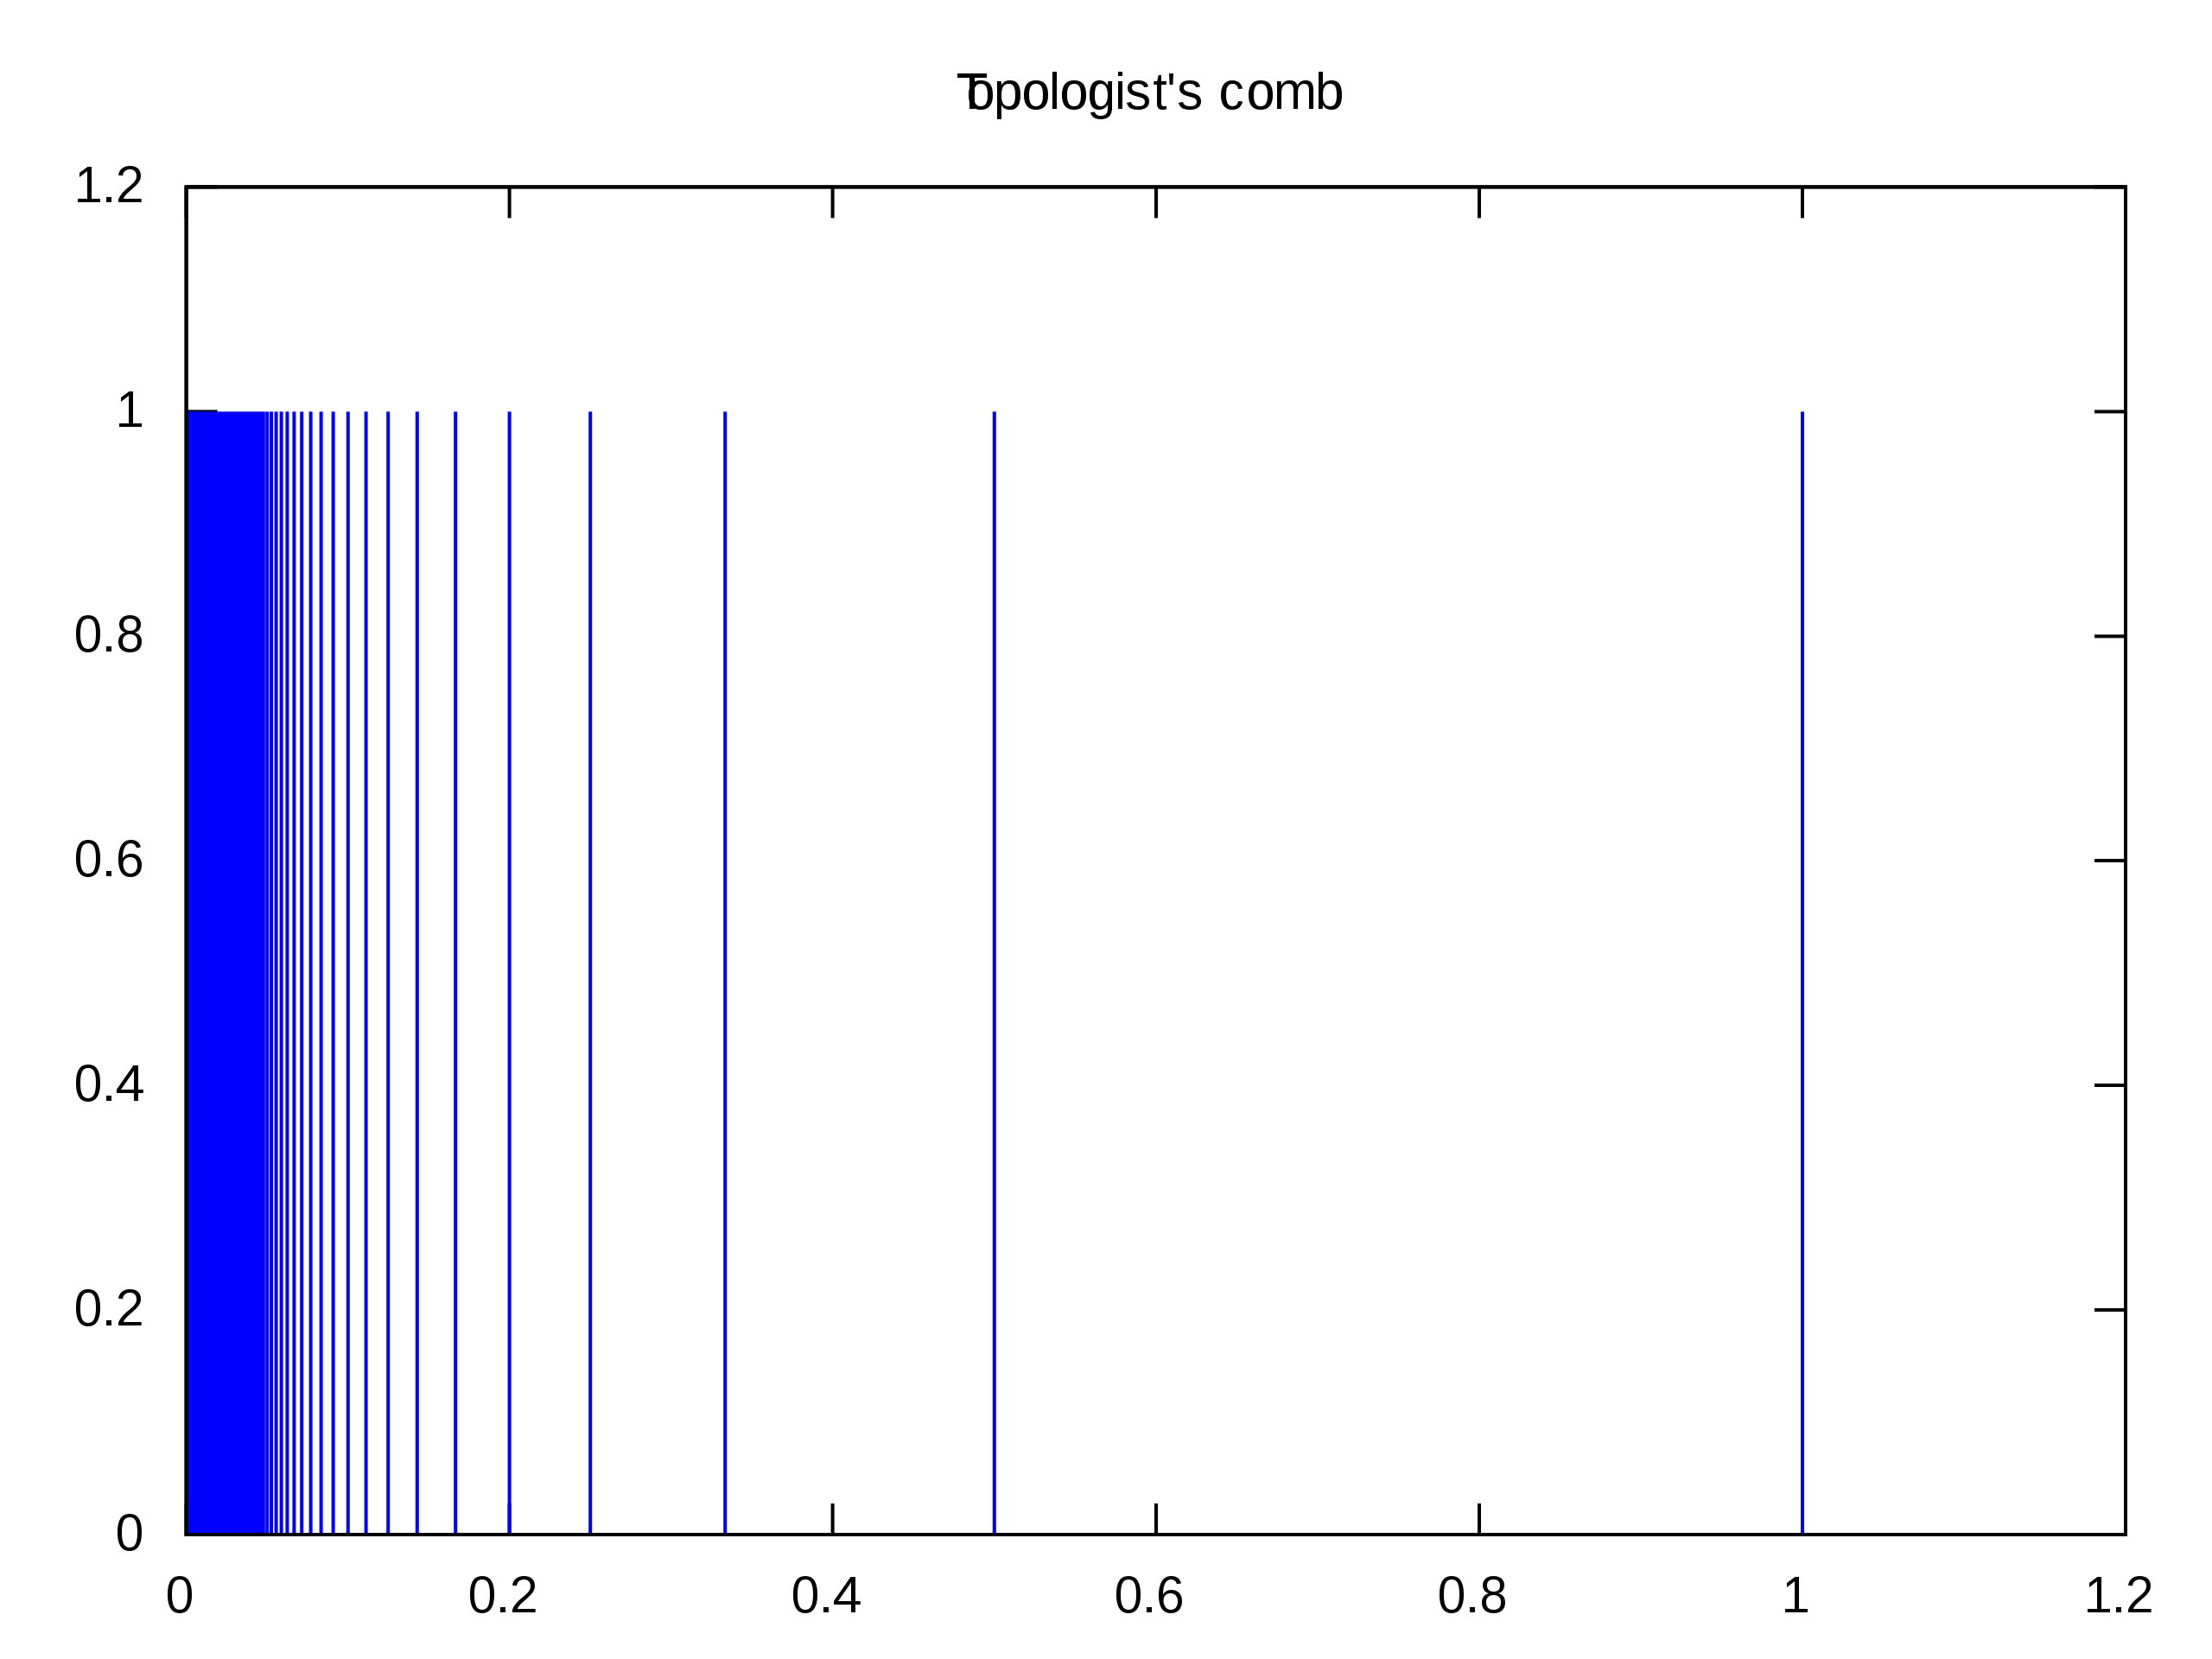
\includegraphics[width=10cm]{images/m4_comb.png}
\caption{\small{Comb space}}
\label{img:combspace}
\end{figure}
So, none of the three assumptions for a universal covering are redundant.
\end{document}